% =============================================================================
% Sustainome — slides in the midcentury-olive style (recreated; the original
% tdstyle.tex / theme .sty are not public, so the look is rebuilt here from the
% Overleaf preview: olive band, cream paper, EB Garamond small caps titles,
% Montserrat body).  Compile with XeLaTeX, twice:
%     xelatex Sustainome_Slides.tex && xelatex Sustainome_Slides.tex
% =============================================================================
\documentclass[aspectratio=169,10pt]{beamer}

\usepackage{fontspec}
\usepackage{tcolorbox}
\tcbuselibrary{skins, raster}
\usepackage{booktabs}
\usepackage{array}
\usepackage{pgfplots}
\pgfplotsset{compat=1.18}
\usetikzlibrary{positioning, arrows.meta, fit, backgrounds}
\usepackage{pifont}

% ---------------------------------------------------------------- fonts
\setsansfont{Montserrat-Regular.otf}[
  BoldFont=Montserrat-SemiBold.otf, ItalicFont=Montserrat-Italic.otf,
  BoldItalicFont=Montserrat-SemiBoldItalic.otf]
\newfontfamily\garamond{EBGaramond-Regular.otf}[
  ItalicFont=EBGaramond-Italic.otf, BoldFont=EBGaramond-SemiBold.otf]
\usefonttheme{professionalfonts}

% ---------------------------------------------------------------- colours
\definecolor{oliveGreen}{HTML}{5A7411}
\definecolor{oliveLight}{HTML}{B5C194}
\definecolor{olivePaper}{HTML}{F8F6F2}
\definecolor{oliveInk}{HTML}{2E2F2A}
\definecolor{oliveRust}{HTML}{A9532B}
\definecolor{oliveGrey}{HTML}{A3A39B}

% ---------------------------------------------------------------- theme
\setbeamertemplate{navigation symbols}{}
\setbeamercolor{background canvas}{bg=olivePaper}
\setbeamercolor{normal text}{fg=oliveInk}
\setbeamercolor{structure}{fg=oliveGreen}
\setbeamercolor{alerted text}{fg=oliveRust}
\setbeamertemplate{itemize items}[square]
\setbeamerfont{normal text}{size=\small}

\setbeamertemplate{frametitle}{%
  \nointerlineskip
  \begin{beamercolorbox}[wd=\paperwidth,ht=8.5mm,dp=3.5mm,leftskip=6mm]{frametitlebox}
    {\garamond\scshape\fontsize{15}{17}\selectfont\insertframetitle}
  \end{beamercolorbox}\vspace{2mm}}
\setbeamercolor{frametitlebox}{bg=oliveGreen,fg=white}

\setbeamertemplate{footline}{%
  \begin{tikzpicture}[remember picture,overlay]
    \fill[oliveGreen] (current page.south west) rectangle
      ([xshift={\paperwidth*\insertframenumber/\inserttotalframenumber}, yshift=0.6mm]current page.south west);
  \end{tikzpicture}%
  \leavevmode\hbox to \paperwidth{\hspace{6mm}%
    {\fontsize{5.5}{6}\selectfont\color{oliveGrey}Group 13\hfill Sustainome · BIO544\hfill
     \insertframenumber/\inserttotalframenumber}\hspace{6mm}}\vspace{2.6mm}}

\setbeamertemplate{title page}{%
  \begin{tikzpicture}[remember picture,overlay]
    % left olive panel + light stripe
    \fill[oliveGreen] (current page.north west) rectangle ([xshift=0.60\paperwidth]current page.south west);
    \fill[oliveLight] ([xshift=0.60\paperwidth]current page.north west) rectangle ([xshift=0.612\paperwidth]current page.south west);
    % left text block
    \node[anchor=north west, text=white, text width=0.50\paperwidth, align=left, inner sep=0pt]
      at ([xshift=9mm, yshift=-11mm]current page.north west) {%
      {\fontsize{6.5}{8}\selectfont\color{oliveLight}BIO544 COMPUTATIONAL GASTRONOMY · MONSOON 2026}\\[7mm]
      {\garamond\scshape\fontsize{38}{40}\selectfont\inserttitle}\\[3mm]
      {\garamond\itshape\fontsize{13}{16}\selectfont\insertsubtitle}\\[5mm]
      {\color{oliveLight}\rule{18mm}{0.8pt}}\\[4mm]
      {\fontsize{9}{12}\selectfont Do greener food swaps really keep the nutrition?\\
       We joined France's nutrition and life-cycle databases to find out.}\\[9mm]
      {\garamond\fontsize{13}{15}\selectfont\insertauthor}};
    % right panel: key numbers
    \foreach \y/\n/\l in {0/2{,}272/foods joined exactly,
                          1/4.5\%/of greenest swaps keep the nutrition,
                          2/38–82\%/less CO\textsubscript{2}e in redesigned meals,
                          3/6 of 9/claims robust to every test}{
      \node[anchor=north west, text width=0.30\paperwidth, align=left, inner sep=0pt]
        at ([xshift=0.655\paperwidth, yshift={-11mm-\y*16.5mm}]current page.north west) {%
        {\garamond\fontsize{22}{23}\selectfont\color{oliveGreen}\n}\\[0.5mm]
        {\hyphenpenalty=10000\fontsize{6.8}{8.5}\selectfont\color{oliveInk!75}\l}};
      \draw[oliveGrey!50, line width=0.4pt]
        ([xshift=0.655\paperwidth, yshift={-24.5mm-\y*16.5mm}]current page.north west) --
        ++(0.29\paperwidth,0);}
    \node[anchor=south west, text width=0.30\paperwidth, align=left, inner sep=0pt]
      at ([xshift=0.655\paperwidth, yshift=7mm]current page.south west)
      {\fontsize{6}{7.5}\selectfont\color{oliveInk!60}CIQUAL 2025 × AGRIBALYSE 3.2};
  \end{tikzpicture}}

% section divider: \tdsection{title}{subtitle}
\newcommand{\tdsubtitle}{}
\newcommand{\tdsection}[2]{\renewcommand{\tdsubtitle}{#2}\section{#1}}
\setbeamertemplate{section page}{%
  \begin{tikzpicture}[remember picture,overlay]
    \fill[oliveGreen] (current page.north west) rectangle ([xshift=2.2mm]current page.south west);
    \fill[oliveLight] ([xshift=2.2mm]current page.north west) rectangle ([xshift=3.6mm]current page.south west);
  \end{tikzpicture}%
  \vspace*{12mm}\hspace*{10mm}\begin{minipage}{0.8\paperwidth}
    {\fontsize{7}{8}\selectfont\color{oliveGreen!70}\MakeUppercase{Section \insertsectionnumber}}\par\vspace{4mm}
    {\garamond\fontsize{24}{27}\selectfont\color{oliveGreen}\insertsectionhead}\par\vspace{5mm}
    {\small\color{oliveInk!70}\tdsubtitle}
  \end{minipage}}


% ---------------------------------------------------------------- helpers (preamble only)
\newcommand{\ac}[1]{\textcolor{oliveGreen}{#1}}
\newcommand{\acb}[1]{\textcolor{oliveGreen}{\textbf{#1}}}
\newcommand{\code}[1]{\texttt{#1}}
\newcommand{\thead}[1]{{\fontsize{6.5}{8}\selectfont\color{oliveInk!70}\MakeUppercase{#1}}}
\newcommand{\aside}[1]{\par\vspace{0pt plus 1fill}{\color{oliveGrey!80}\rule{\linewidth}{0.4pt}}\par
  {\scriptsize\color{oliveInk!65}#1\par}}
\newcommand{\srcline}[1]{\noindent\hangindent=1.0em\hangafter=1
  \textcolor{oliveGreen}{\textbullet}\hspace{0.5em}#1\par}
% big number with caption
\newcommand{\num}[3][oliveGreen]{{\centering{\fontsize{20}{22}\selectfont\bfseries\color{#1}#2}\par
  \vspace{1pt}{\scriptsize\color{oliveInk!75}#3}\par}}
\newcommand{\yes}{\textcolor{oliveGreen}{\ding{51}}}
\newcommand{\no}{\textcolor{oliveRust}{\ding{55}}}
\newcommand{\partly}{\textcolor{oliveGrey}{$\sim$}}
\newcommand{\na}{\textcolor{oliveGrey}{--}}
% card rows: stepflow{n} with \stepcard{title}{text} and \steparrow
\newenvironment{stepflow}[1]{\def\stepn{#1}\noindent\begin{tikzpicture}[x=1mm,y=1mm]\def\stepx{0}}{\end{tikzpicture}\par}
\newcommand{\stepcard}[3][1]{%
  \pgfmathsetmacro{\stepw}{#1*(142-(\stepn-1)*7)/\stepn}%
  \draw[oliveGreen, line width=0.9pt] (\stepx,0) -- ++(\stepw,0);
  \node[anchor=north west, text width=\stepw mm, inner sep=0pt, align=left] at (\stepx,-2)
    {\textbf{\small #2}\\[1pt]{\scriptsize\color{oliveInk!80}#3}};
  \pgfmathsetmacro{\stepx}{\stepx+\stepw}\xdef\stepx{\stepx}}
\newcommand{\steparrow}{%
  \node[oliveGrey] at (\stepx+3.5,-5) {$\rightarrow$};
  \pgfmathsetmacro{\stepx}{\stepx+7}\xdef\stepx{\stepx}}

\pgfplotsset{
  oaxis/.style={axis line style={oliveGrey}, tick style={oliveGrey}, tick label style={font=\scriptsize},
    label style={font=\scriptsize}, legend style={font=\scriptsize, draw=none, fill=none},
    every node near coord/.append style={font=\scriptsize\bfseries}},
}

\title[Sustainome]{Sustainome}
\subtitle{The sustainable plate frontier: nutrient–environment trade-offs and food substitution}
\author[Group 13]{Group 13}
\institute{BIO544 Computational Gastronomy · Monsoon 2026}
\date{Data: ANSES-CIQUAL 2025 × AGRIBALYSE 3.2}

\begin{document}

\begin{frame}[plain]
  \titlepage
\end{frame}

% =============================================================================

\begin{frame}{Do greener food swaps keep the nutrition?}

  \acb{Footprint rankings compare foods per kilogram; nutrition scores ignore the
  planet.} A swap only helps if the replacement does the same nutritional job — so we
  tested exactly that, at the level of single foods, pairs of foods and whole meals.

  \vspace{4mm}
  \begin{columns}[T]
    \column{0.24\textwidth}\num{2,272}{foods with nutrients \emph{and} impacts}
    \column{0.24\textwidth}\num{15}{nutrients}
    \column{0.24\textwidth}\num{7}{environmental indicators}
    \column{0.24\textwidth}\num{3}{units: per 100 g, 100 kcal, 10 g protein}
  \end{columns}

  \aside{Data: ANSES-CIQUAL 2025 (3,484 foods, nutrient composition) joined to
  AGRIBALYSE 3.2 (life-cycle impacts, EU Environmental Footprint method) on the shared
  CIQUAL food code. Average products eaten in France; not diet advice.}

\end{frame}

\begin{frame}{What we did, and why it is useful}

  \begin{stepflow}{3}
    \stepcard{The problem}{Labels such as Nutri-Score or Green-Score grade one product at
      a time. Nobody checks whether the “greener” replacement still gives the same
      protein, B12 or zinc.}
    \steparrow
    \stepcard{What we did}{Joined nutrition and life-cycle data for 2,272 foods, built a
      nutrient-equivalence test for every swap, optimised whole meals, and stress-tested
      every claim.}
    \steparrow
    \stepcard{Why it is useful}{It shows which green swaps are real (156) and which
      mislead (37,280), how much a meal can really save (38–82\%), and what that costs
      (more water in 3 of 5 meals).}
  \end{stepflow}

  \vspace{20mm}
  {\small\acb{A label tells you a grade. We tell you whether a swap actually works.}
  The evidence could feed “greener equivalent” suggestions in labels and apps, and
  diet advice that must not lose nutrients.\par}

\end{frame}

\begin{frame}{Five deliverables, from data to validation}

  \begin{stepflow}{5}
    \stepcard{D1 · data}{2,272 foods joined exactly}
    \steparrow
    \stepcard{D2 · foods}{best trade-offs in 3 units}
    \steparrow
    \stepcard{D3 · pairs}{which swaps keep nutrition}
    \steparrow
    \stepcard{D4 · meals}{optimise whole meals}
    \steparrow
    \stepcard{D5 · checks}{do claims survive?}
  \end{stepflow}

  \vspace{14mm}
  {\small\acb{Each level answers a different question.} D2 asks which single foods sit on the
  best nutrition–environment frontier; D3 whether one food can replace another; D4 how
  several foods should change together; D5 whether any of it survives other reasonable
  assumptions.\par}

  \aside{Each deliverable has its own outputs and pass/fail acceptance criteria: 33 of 33
  met. One command rebuilds every result from the frozen raw files.}

\end{frame}

% =============================================================================

\begin{frame}{D1 · 2,272 foods joined exactly}

  \begin{columns}[c]
    \column{0.62\textwidth}
    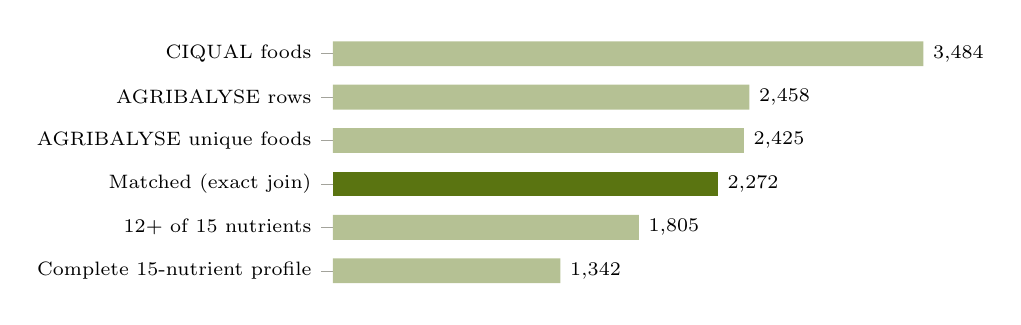
\begin{tikzpicture}
    \begin{axis}[oaxis, xbar, bar width=9pt, width=\linewidth, height=5.0cm, xmin=0, xmax=4900,
        ytick={1,...,6}, yticklabels={Complete 15-nutrient profile, 12+ of 15 nutrients, Matched (exact join),
          AGRIBALYSE unique foods, AGRIBALYSE rows, CIQUAL foods},
        axis x line=none, axis y line*=left, y axis line style={draw=none}, enlarge y limits=0.12,
        nodes near coords, point meta=rawx, nodes near coords align={horizontal},
        every node near coord/.append style={/pgf/number format/1000 sep={\mathord{,}}}]
      \addplot[fill=oliveLight, draw=none, bar shift=0pt] coordinates {(1342,1) (1805,2) (2425,4) (2458,5) (3484,6)};
      \addplot[fill=oliveGreen, draw=none, bar shift=0pt] coordinates {(2272,3)};
    \end{axis}
    \end{tikzpicture}
    \column{0.36\textwidth}
    \num{93.69\%}{of AGRIBALYSE foods matched}\vspace{2mm}
    \num{33}{duplicate rows resolved by one tested rule}\vspace{2mm}
    \num[oliveRust]{0}{missing values set to zero}
  \end{columns}

  \aside{\acb{No name guessing:} names were only used to audit the join. Missing stays
  missing; “traces” = 0; “below limit x” = x/2 (alternatives re-tested in D5).}

\end{frame}

% =============================================================================

\begin{frame}{D2 · The protein gap shrinks but never flips}

  \begin{columns}[c]
    \column{0.66\textwidth}
    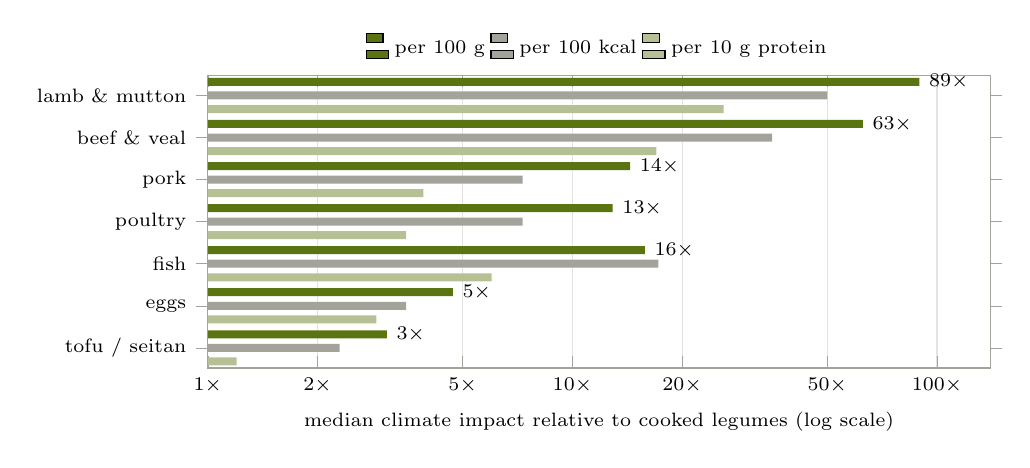
\begin{tikzpicture}
    \begin{axis}[oaxis, xbar, xmode=log, width=0.95\linewidth, height=5.3cm, bar width=2.9pt,
        xmin=1, xmax=140, ytick={1,...,7},
        yticklabels={tofu / seitan, eggs, fish, poultry, pork, beef \& veal, lamb \& mutton},
        xtick={1,2,5,10,20,50,100}, xticklabels={1$\times$,2$\times$,5$\times$,10$\times$,20$\times$,50$\times$,100$\times$},
        xlabel={median climate impact relative to cooked legumes (log scale)},
        xmajorgrids, grid style={oliveGrey!30}, enlarge y limits=0.08,
        legend style={at={(0.5,1.02)}, anchor=south, legend columns=3}, reverse legend]
      \addplot[fill=oliveLight, draw=none] coordinates {(1.2,1) (2.9,2) (6.0,3) (3.5,4) (3.9,5) (17.0,6) (26.0,7)};
      \addplot[fill=oliveGrey, draw=none] coordinates {(2.3,1) (3.5,2) (17.2,3) (7.3,4) (7.3,5) (35.3,6) (50.0,7)};
      \addplot[fill=oliveGreen, draw=none, nodes near coords, point meta=rawx, nodes near coords align={horizontal},
          nodes near coords={\pgfmathprintnumber[fixed,precision=0]{\pgfplotspointmeta}$\times$}]
          coordinates {(3.1,1) (4.7,2) (15.8,3) (12.9,4) (14.4,5) (62.6,6) (89.4,7)};
      \legend{per 10 g protein, per 100 kcal, per 100 g}
    \end{axis}
    \end{tikzpicture}
    \column{0.32\textwidth}
    {\centering\scriptsize Beef \& veal vs cooked legumes\par}\vspace{2mm}
    \num{63$\times$}{per 100 g}\vspace{1mm}
    \num[oliveGrey!80!black]{35$\times$}{per 100 kcal}\vspace{1mm}
    \num[oliveLight!60!black]{17$\times$}{per 10 g protein}
  \end{columns}

  \aside{\acb{Why it matters:} the measuring unit changes the size of the gap, never its
  direction. Bootstrap intervals stay above 1 for every animal category in every unit.}

\end{frame}

\begin{frame}{D2 · Nutrition and climate often conflict}

  \begin{columns}[c]
    \column{0.62\textwidth}
    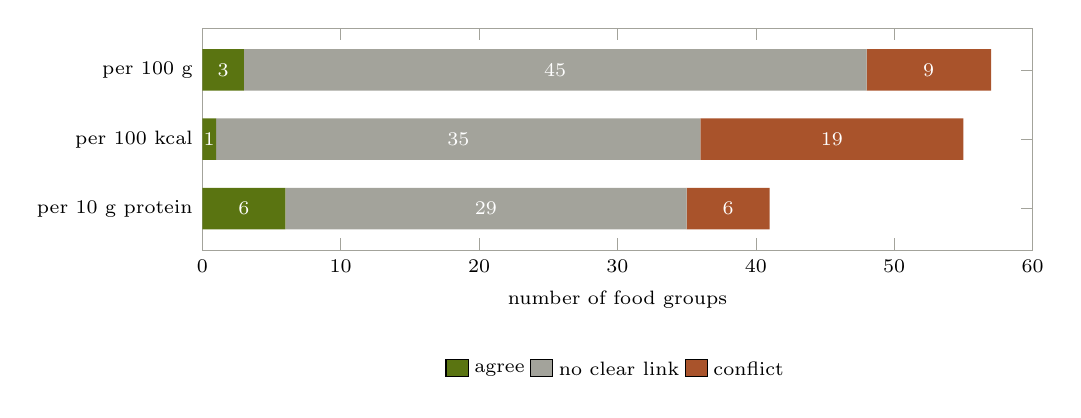
\begin{tikzpicture}
    \begin{axis}[oaxis, xbar stacked, bar width=15pt, width=\linewidth, height=4.4cm, xmin=0, xmax=60,
        ytick={1,2,3}, yticklabels={per 10 g protein, per 100 kcal, per 100 g}, enlarge y limits=0.3,
        xlabel={number of food groups},
        nodes near coords, legend style={at={(0.5,-0.45)}, anchor=north, legend columns=3},
        every node near coord/.append style={white}]
      \addplot[fill=oliveGreen, draw=none] coordinates {(6,1) (1,2) (3,3)};
      \addplot[fill=oliveGrey, draw=none] coordinates {(29,1) (35,2) (45,3)};
      \addplot[fill=oliveRust, draw=none] coordinates {(6,1) (19,2) (9,3)};
      \legend{agree, no clear link, conflict}
    \end{axis}
    \end{tikzpicture}
    \column{0.36\textwidth}
    \num[oliveRust]{19 vs 1}{groups conflict vs agree, per 100 kcal}\vspace{2mm}
    \num{0.61}{overlap of “efficient” foods, per 100 g vs per 100 kcal}\vspace{2mm}
    \num{25\%}{of food pairs flip climate order between units}
  \end{columns}

  \aside{\acb{Why it matters:} healthy and green often pull apart inside a food group, so a
  swap cannot be judged on climate alone. 1,045 foods in 55 groups per 100 kcal.}

\end{frame}

% =============================================================================

\begin{frame}{D3 · Nutrients alone rebuild the food map}

  \begin{columns}[c]
    \column{0.5\textwidth}
    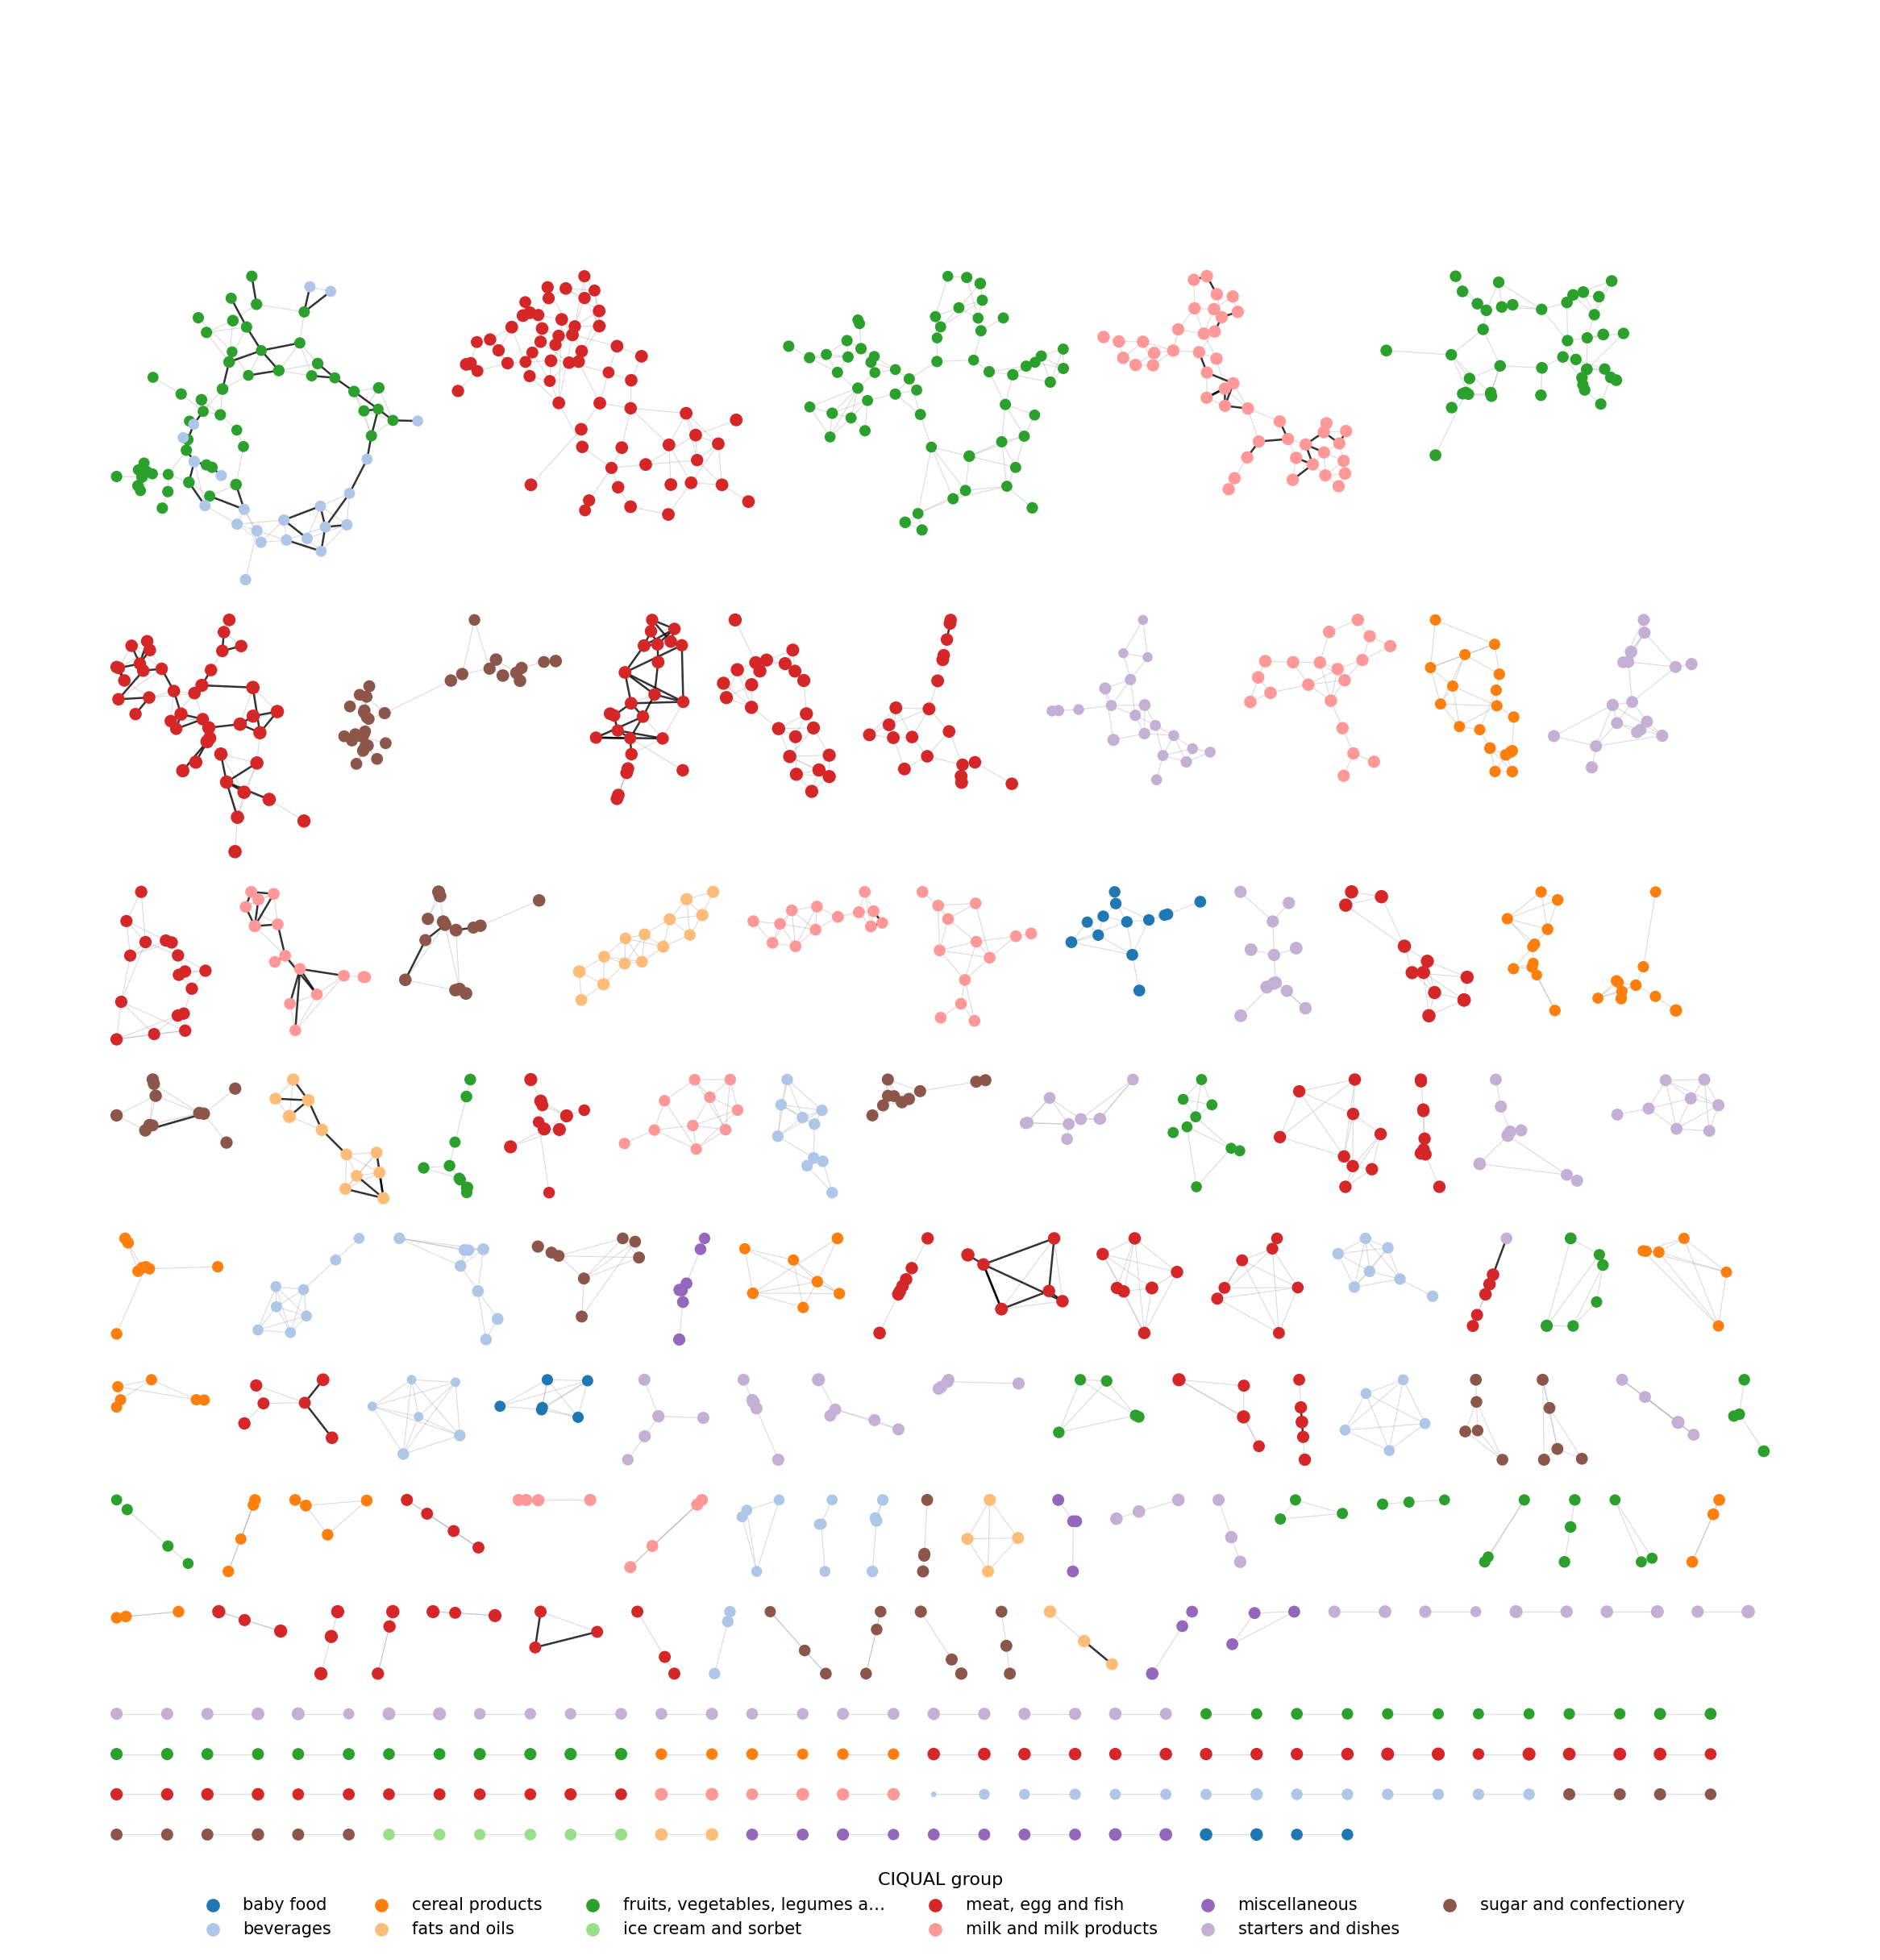
\includegraphics[width=0.78\linewidth]{presentation/assets/d3_network.png}
    \column{0.48\textwidth}
    {\small Two foods are linked only if each is among the other's 5 closest matches on a
    15-nutrient profile, within a threshold fixed in advance ($\tau = 0.236$).\par}
    \vspace{3mm}
    \begin{columns}[T]
      \column{0.5\linewidth}\num{1,805}{foods}\vspace{1mm}\num{180}{communities}
      \column{0.5\linewidth}\num{1,736}{links}\vspace{1mm}\num{0.90}{NMI with official groups}
    \end{columns}
  \end{columns}

  \aside{\acb{No leakage:} the network never sees environmental data; shuffling every impact
  column leaves the links unchanged.}

\end{frame}

\begin{frame}{D3 · Only 4.5\% of “greenest swaps” keep the nutrition}

  \begin{columns}[c]
    \column{0.38\textwidth}
    \centering{\fontsize{40}{42}\selectfont\bfseries\color{oliveRust}4.5\%}\par\vspace{1mm}
    {\scriptsize of “greenest swaps” keep the nutrition (732 foods)\par}\vspace{4mm}
    \num{70\% $\rightarrow$ 0\%}{median climate gain once equivalence is required}
    \column{0.6\textwidth}
    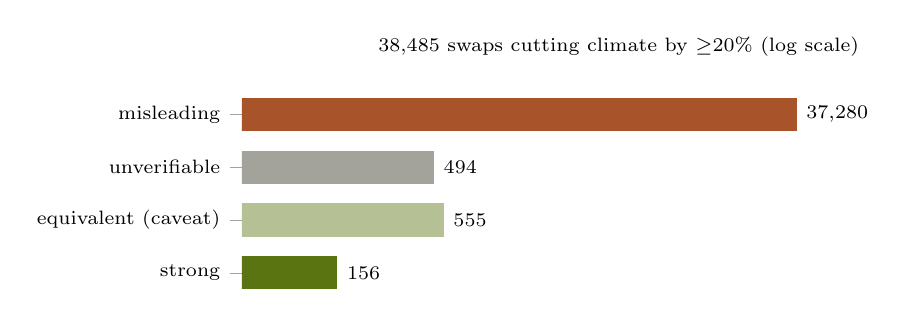
\begin{tikzpicture}
    \begin{axis}[oaxis, xbar, xmode=log, width=0.92\linewidth, height=4.4cm, bar width=12pt, xmin=50, xmax=400000,
        ytick={1,2,3,4}, yticklabels={strong, equivalent (caveat), unverifiable, misleading},
        axis x line=none, axis y line*=left, y axis line style={draw=none}, enlarge y limits=0.2,
        nodes near coords, point meta=rawx, nodes near coords align={horizontal},
        every node near coord/.append style={/pgf/number format/1000 sep={\mathord{,}}},
        title={\scriptsize 38,485 swaps cutting climate by $\geq$20\% (log scale)}]
      \addplot[fill=oliveGreen, draw=none, bar shift=0pt] coordinates {(156,1)};
      \addplot[fill=oliveLight, draw=none, bar shift=0pt] coordinates {(555,2)};
      \addplot[fill=oliveGrey, draw=none, bar shift=0pt] coordinates {(494,3)};
      \addplot[fill=oliveRust, draw=none, bar shift=0pt] coordinates {(37280,4)};
    \end{axis}
    \end{tikzpicture}
  \end{columns}

  \aside{\acb{Equivalent} = close nutrient profile \emph{and} keeps $\geq$80\% protein,
  energy 0.67–1.5$\times$, $\geq$50\% of each key micronutrient, $\leq$1.25$\times$ salt,
  saturated fat and sugars. \acb{Strong} = also reliable data and no rise in land or water.}

\end{frame}

\begin{frame}{D3 · Real swaps and misleading swaps, checked by hand}

  {\footnotesize
  \begin{tabular}{@{}>{\raggedright\arraybackslash}p{5.4cm}
                    >{\raggedright\arraybackslash}p{1.8cm}
                    >{\raggedright\arraybackslash}p{1.9cm}
                    >{\raggedright\arraybackslash}p{4.4cm}@{}}
    \toprule
    \thead{swap, gram for gram} & \thead{climate cut} & \thead{verdict} & \thead{why} \\
    \midrule
    \textbf{Hazelnut oil $\rightarrow$ rapeseed oil} & $-$75\% & \ac{strong} & nutrient distance 0.03 \\
    \textbf{Peanut oil $\rightarrow$ olive oil} & $-$62\% & \ac{strong} & nutrient distance 0.02 \\
    \textbf{Roast veal $\rightarrow$ roast turkey} & $-$83\% & \ac{strong} & same role, similar profile \\
    \textbf{Mushroom soup $\rightarrow$ tomato soup} & $-$85\% & \ac{strong} & nutrient distance 0.12 \\
    \midrule
    \textbf{Beef chuck $\rightarrow$ haricot beans} & $-$99\% & \textcolor{oliveRust}{misleading} & loses protein, energy, zinc, B12 \\
    \textbf{Chicken leg $\rightarrow$ haricot beans} & $-$95\% & \textcolor{oliveRust}{misleading} & loses protein, energy, zinc, B12 \\
    \textbf{Merguez $\rightarrow$ tofu sausage} & $-$96\% & \textcolor{oliveRust}{misleading} & loses protein, potassium, zinc \\
    \bottomrule
  \end{tabular}\par}

  \vspace{3mm}
  {\small\acb{Most common failures:} protein (15,869 swaps), energy (14,727), B12 (11,347),
  zinc (10,915). Meat-to-plant swaps need compensation at meal level — that is D4.\par}

  \aside{30 swaps audited by hand: 20 culinarily plausible, all 10 sampled misleading swaps
  confirmed. Caveat found: linseed oil's omega-3 is outside our 15 nutrients.}

\end{frame}

% =============================================================================

\begin{frame}{D4 · Whole meals: 38–82\% less climate impact}

  \begin{columns}[c]
    \column{0.64\textwidth}
    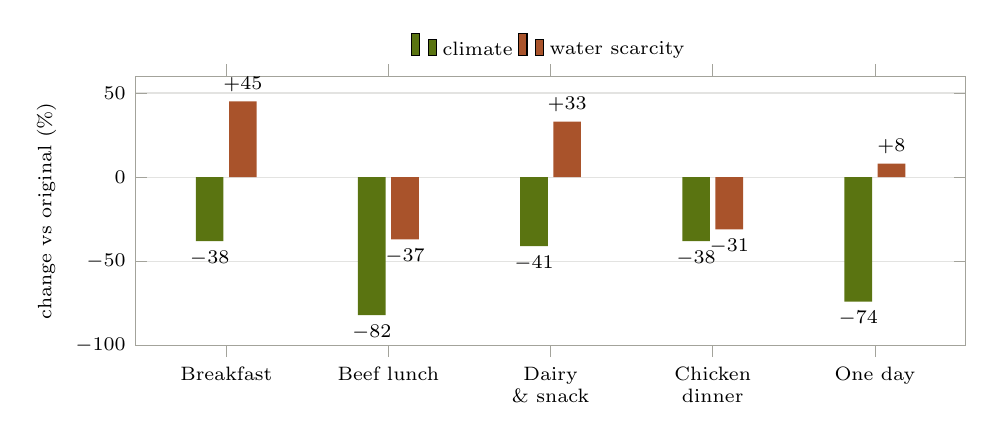
\begin{tikzpicture}
    \begin{axis}[oaxis, ybar, width=\linewidth, height=5.0cm, bar width=10pt, ymin=-100, ymax=60,
        xtick={1,...,5}, xticklabels={Breakfast, Beef lunch, Dairy \& snack, Chicken dinner, One day},
        enlarge x limits=0.14, x tick label style={align=center, text width=1.3cm},
        ylabel={change vs original (\%)}, ymajorgrids, grid style={oliveGrey!30},
        nodes near coords, point meta=rawy,
        nodes near coords={\pgfmathprintnumber[showpos]{\pgfplotspointmeta}},
        legend style={at={(0.5,1.02)}, anchor=south, legend columns=2}]
      \addplot[fill=oliveGreen, draw=none] coordinates {(1,-38) (2,-82) (3,-41) (4,-38) (5,-74)};
      \addplot[fill=oliveRust, draw=none] coordinates {(1,45) (2,-37) (3,33) (4,-31) (5,8)};
      \legend{climate, water scarcity}
    \end{axis}
    \end{tikzpicture}
    \column{0.34\textwidth}
    {\scriptsize The optimiser chooses grams of foods in each meal slot. It must keep energy
    within $\pm$5\%, protein $\geq$95\%, fibre and 7 micronutrients $\geq$90\%, and salt,
    saturated fat and sugars $\leq$ the original.\par}
    \vspace{3mm}
    \num[oliveRust]{3 of 5}{meals use \emph{more} water}
  \end{columns}

  \aside{\acb{Why it matters:} large cuts are possible at meal level, but optimising climate
  alone can shift the burden to water. Shown: the operating point declared before solving
  (nutrient deviation $\leq$0.10, $\leq$50\% of grams changed).}

\end{frame}

\begin{frame}{D4 · Savings per meal, step by step}

  {\footnotesize
  \begin{tabular}{@{}>{\raggedright\arraybackslash}p{2.3cm}
                    >{\raggedleft\arraybackslash}p{1.3cm}
                    >{\raggedleft\arraybackslash}p{1.5cm}
                    >{\raggedleft\arraybackslash}p{1.5cm}
                    >{\raggedleft\arraybackslash}p{1.8cm}
                    >{\raggedleft\arraybackslash}p{1.6cm}
                    >{\raggedleft\arraybackslash}p{2.3cm}@{}}
    \toprule
    \thead{meal} & \thead{kg CO\textsubscript{2}e} & \thead{portions only} & \thead{1 new food}
      & \thead{same profile (D = 0)} & \thead{operating point} & \thead{no nutrition rules} \\
    \midrule
    \textbf{Breakfast} & 0.89 & $-$10\% & $-$22\% & $-$19\% & \acb{$-$38\%} & $-$67\% (8 broken) \\
    \textbf{Beef lunch} & 5.04 & $-$13\% & $-$23\% & $-$68\% & \acb{$-$82\%} & $-$93\% (8) \\
    \textbf{Dairy \& snack} & 1.26 & $-$9\% & $-$29\% & $-$28\% & \acb{$-$41\%} & $-$68\% (8) \\
    \textbf{Chicken dinner} & 1.52 & $-$9\% & $-$12\% & $-$19\% & \acb{$-$38\%} & $-$84\% (4) \\
    \textbf{One day} & 7.45 & $-$17\% & $-$38\% & $-$65\% & \acb{$-$74\%} & $-$88\% (6) \\
    \bottomrule
  \end{tabular}\par}

  \vspace{4mm}
  {\small\acb{Read it left to right:} changing portions alone saves 9–17\%; letting the meal
  change within the declared limits saves 38–82\%. Removing the nutrition rules saves more,
  but breaks 4–8 of them — \ac{the rules, not the objective, protect nutrition}.\par}

  \aside{Only 0.3–7.7\% of 5,000 random like-for-like swaps meet all rules. Every optimiser
  solution is re-checked against every rule. Solver: HiGHS via SciPy.}

\end{frame}

\begin{frame}{D4 · A few well-chosen swaps do most of the work}

  \begin{columns}[c]
    \column{0.64\textwidth}
    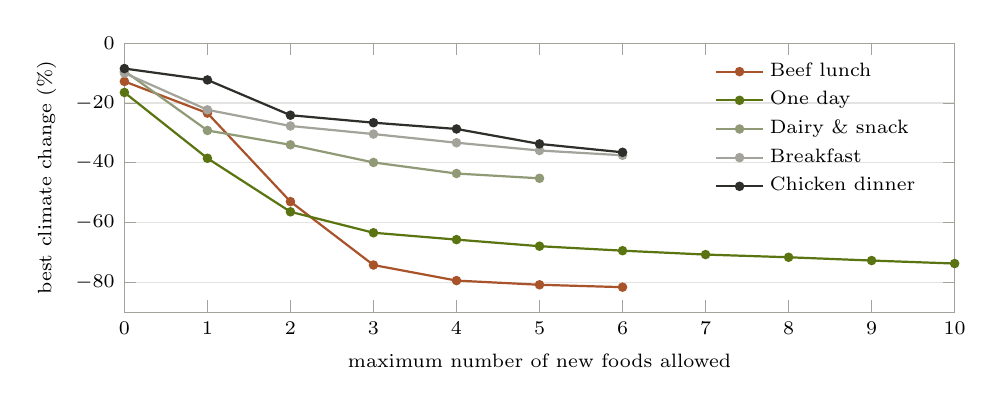
\begin{tikzpicture}
    \begin{axis}[oaxis, width=\linewidth, height=5.0cm, xmin=0, xmax=10, ymin=-90, ymax=0,
        xlabel={maximum number of new foods allowed}, ylabel={best climate change (\%)},
        ymajorgrids, grid style={oliveGrey!30}, legend pos=north east, legend cell align=left,
        every axis plot/.append style={thick, mark=*, mark size=1.3pt}]
      \addplot[oliveRust] coordinates {(0,-12.8) (1,-23.4) (2,-53.0) (3,-74.2) (4,-79.4) (5,-80.8) (6,-81.6)};
      \addplot[oliveGreen] coordinates {(0,-16.5) (1,-38.5) (2,-56.4) (3,-63.4) (4,-65.7) (5,-67.9) (6,-69.4) (7,-70.7) (8,-71.6) (9,-72.7) (10,-73.7)};
      \addplot[oliveLight!80!black] coordinates {(0,-9.3) (1,-29.2) (2,-34.0) (3,-39.9) (4,-43.6) (5,-45.2)};
      \addplot[oliveGrey] coordinates {(0,-10.0) (1,-22.3) (2,-27.7) (3,-30.4) (4,-33.3) (5,-35.9) (6,-37.5)};
      \addplot[oliveInk] coordinates {(0,-8.5) (1,-12.3) (2,-24.1) (3,-26.6) (4,-28.7) (5,-33.7) (6,-36.5)};
      \legend{Beef lunch, One day, Dairy \& snack, Breakfast, Chicken dinner}
    \end{axis}
    \end{tikzpicture}
    \column{0.34\textwidth}
    \num[oliveRust]{$-$74\%}{beef lunch with 3 new foods (portions only: $-$13\%)}\vspace{3mm}
    {\scriptsize Example: the 120 g steak becomes about 82 g textured soy protein and 54 g
    roast turkey; some pasta becomes millet.\par}
  \end{columns}

  \aside{Mixed-integer model limiting the number of new foods; nutrient deviation
  $\leq$0.10; solved to a 0.5\% optimality gap. Gains flatten after about five new foods.}

\end{frame}

% =============================================================================

\begin{frame}{D5 · Do the results hold up? 6 of 9 claims are robust}

  \begin{columns}[c]
    \column{0.64\textwidth}
    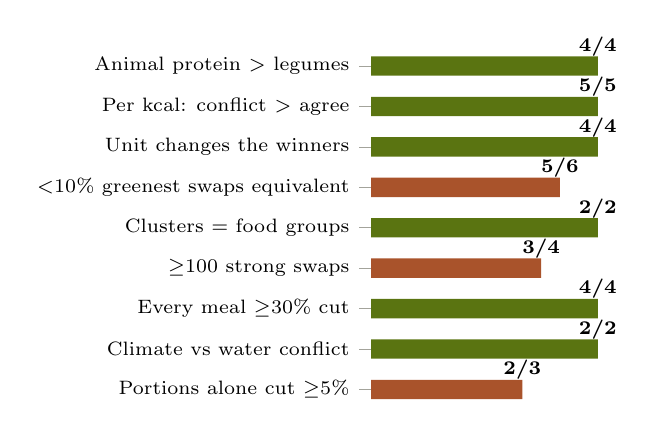
\begin{tikzpicture}
    \begin{axis}[oaxis, xbar, scale only axis, width=3.6cm, height=4.6cm, bar width=7pt, xmin=0, xmax=125,
        ytick={1,...,9}, yticklabels={Portions alone cut $\geq$5\%, Climate vs water conflict, Every meal $\geq$30\% cut,
          $\geq$100 strong swaps, Clusters = food groups, $<$10\% greenest swaps equivalent, Unit changes the winners,
          Per kcal: conflict $>$ agree, Animal protein $>$ legumes},
        axis x line=none, axis y line*=left, y axis line style={draw=none}, enlarge y limits=0.06,
        nodes near coords, point meta=explicit symbolic, nodes near coords align={horizontal}]
      \addplot[fill=oliveGreen, draw=none, bar shift=0pt] coordinates {(100,2)[2/2] (100,3)[4/4] (100,5)[2/2]
          (100,7)[4/4] (100,8)[5/5] (100,9)[4/4]};
      \addplot[fill=oliveRust, draw=none, bar shift=0pt] coordinates {(66.7,1)[2/3] (75,4)[3/4] (83.3,6)[5/6]};
    \end{axis}
    \end{tikzpicture}
    \column{0.34\textwidth}
    \num{6 / 9}{claims robust (green)}\vspace{2mm}
    \num[oliveRust]{3}{conditional — each fails one stated test}\vspace{2mm}
    \num{2.4 pp}{median loss of climate cut under the impact stress test}
  \end{columns}

  \aside{\acb{Tests:} 200 random nutrient weightings, other nutrient sets, a 4 $\times$ 4
  network grid, DQR quality filters, other cleaning rules, B12 rule off, 27 optimiser
  tolerances, bootstrap, DQR-scaled impact shocks. DQR is never treated as a probability.}

\end{frame}

\begin{frame}{D5 · Nine ways a “sustainable” choice fails}

  {\footnotesize
  \begin{tabular}{@{}>{\raggedright\arraybackslash}p{4.4cm}
                    >{\raggedright\arraybackslash}p{9.0cm}@{}}
    \toprule
    \thead{kind of failure} & \thead{example from our data} \\
    \midrule
    \textbf{Greener but not equivalent} & kid meat $\rightarrow$ beans: $-$99\% climate, fails protein, iron, zinc, B12 \\
    \textbf{Ranking flips with the unit} & avocado vs radish: 4.0$\times$ per 100 g, but 0.22$\times$ per 100 kcal \\
    \textbf{Link created by missing data} & two infant formulas: distance 0.08, but 0.58 once gaps are filled \\
    \textbf{Burden shifting} & optimised breakfast: climate $-$38\%, water +45\% \\
    \textbf{Climate-only breaks nutrition} & breakfast without rules: $-$67\%, 8 rules broken \\
    \textbf{Depends on low-quality data} & raw chicory beaten only by foods with DQR $>$ 3 \\
    \textbf{Rests on a known data error} & eggs look efficient; egg impacts flagged as under-estimated \\
    \textbf{Feasible but unrealistic} & 1 g of turkey liver added as a B12 “patch” \\
    \textbf{Variant changes the impact} & mango by plane: 11.60 vs 0.73 kg CO\textsubscript{2}e/kg (16$\times$) \\
    \bottomrule
  \end{tabular}\par}

  \aside{38 cases in total. We kept them in the report rather than hiding them: they show
  exactly where a simple “eat greener” rule goes wrong.}

\end{frame}

% =============================================================================

\begin{frame}{Why it is useful · Compared with existing tools}

  {\footnotesize
  \begin{tabular}{@{}>{\raggedright\arraybackslash}p{4.6cm}
                    >{\centering\arraybackslash}p{1.4cm}
                    >{\centering\arraybackslash}p{1.6cm}
                    >{\centering\arraybackslash}p{1.9cm}
                    >{\centering\arraybackslash}p{1.4cm}
                    >{\raggedright\arraybackslash}p{2.0cm}@{}}
    \toprule
    & \thead{nutrition} & \thead{environment} & \thead{swap checked per nutrient} & \thead{shows trade-offs} & \thead{level} \\
    \midrule
    \textbf{Nutri-Score} & \yes & \no & \no & \no & product \\
    \textbf{Green-Score (ex Eco-Score)} & \no & \yes & \no & \no & product \\
    \textbf{Planet-Score} & \no & \yes & \no & \partly & product \\
    \textbf{Diet optimisation (Perignon 2016)} & \yes & \yes & \na & \yes & whole diet \\
    \textbf{Swap studies (Rose 2022, Grummon 2023)} & \partly & \yes & \partly & \no & diet \\
    \textbf{Recipe networks (Teng 2012)} & \no & \no & \partly & \no & ingredient \\
    \midrule
    \acb{Sustainome} & \yes & \yes & \yes & \yes & \acb{food, pair, meal} \\
    \bottomrule
  \end{tabular}\par}

  \vspace{3mm}
  {\small\acb{The gap we fill:} labels grade one product, studies optimise whole diets; we work
  where the swap decision is made and check nutrition before calling a swap green.\par}

  \aside{\yes\ yes \quad \partly\ partly \quad \no\ no \quad \na\ not applicable — our reading of the published sources.}

\end{frame}

\begin{frame}{Takeaways}

  \begin{columns}[T]
    \column{0.24\textwidth}\num{17$\times$}{beef vs legumes, even per 10 g protein}
    \column{0.24\textwidth}\num[oliveRust]{4.5\%}{of greenest swaps keep the nutrition}
    \column{0.24\textwidth}\num{38–82\%}{meal-level climate cut, nutrition kept}
    \column{0.24\textwidth}\num[oliveRust]{+45\%}{water in one meal: burden shifting}
  \end{columns}

  \vspace{8mm}
  {\centering{\garamond\fontsize{17}{20}\selectfont\color{oliveGreen}Sustainable substitution is real — but conditional.}\par
  \vspace{2mm}{\small check the nutrition · check the unit · check more than climate}\par
  \vspace{6mm}{\garamond\scshape\fontsize{14}{16}\selectfont\color{oliveGreen}Thank you — questions?}\par}

  \aside{Reproducible: 70 automated tests, 33/33 acceptance criteria, one command rebuilds every
  result; independently re-run on Linux with matching results.}

\end{frame}

% =============================================================================
\end{document}
